Overall, the performance of CNN tagger is better than the jet level quantities and their combination in both kinematic regimes considered, $150<\pt<200~\GeV$ and $400<\pt<500~\GeV$.

\begin{figure}[htpb]
\begin{center}
\subfloat[][]{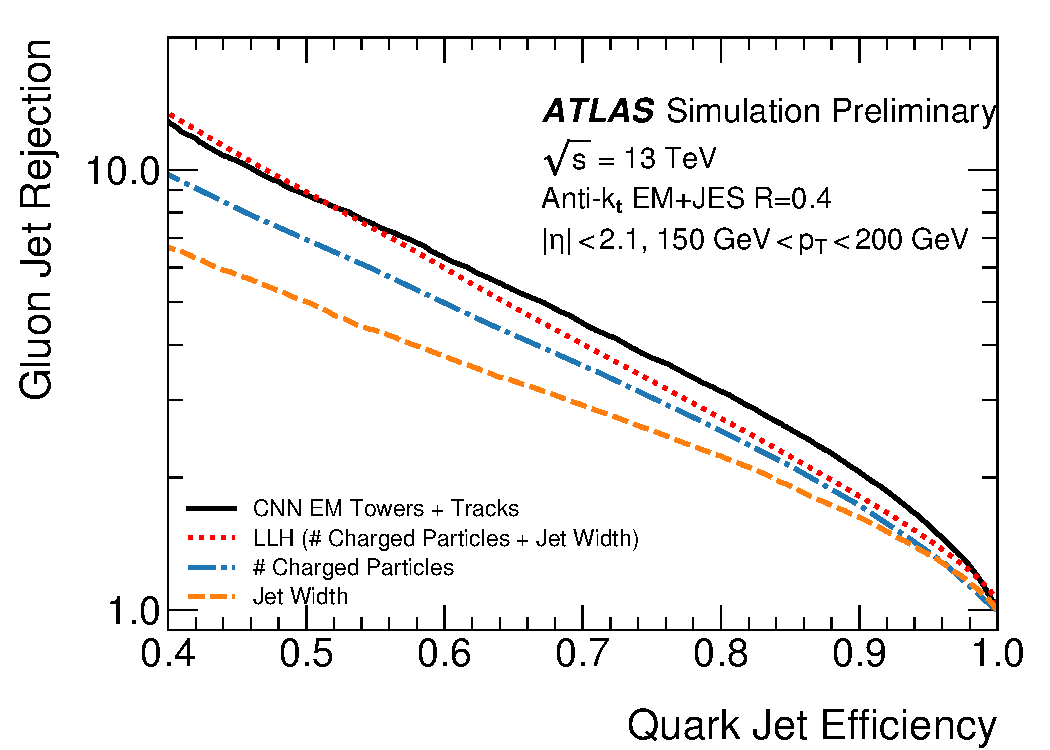
\includegraphics[width=0.5\textwidth]{figures/CNN/ROC_pt150_200_classifier.pdf}\label{lowpt}}
\subfloat[][]{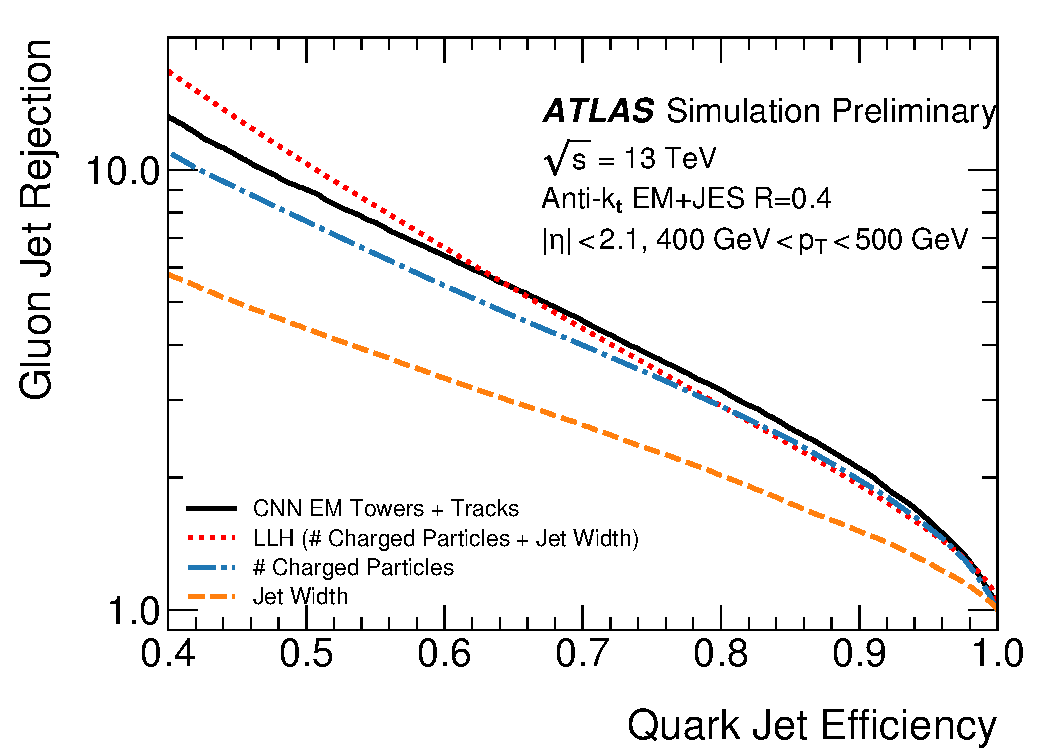
\includegraphics[width=0.5\textwidth]{figures/CNN/ROC_pt400_500_classifier.pdf}\label{highpt}}
\caption{Gluon jet rejection as a function of the quark jet efficiency using physics motivated observables and jet image discriminants
for jets with \protect\subref{lowpt} $150<\pt<200~\GeV$ and \protect\subref{highpt} $400<\pt<500~\GeV$.  The LLH is a tagger constructed from the optimal (likelihood) combination of $n_\text{track}$ and jet width. }
\label{fig:classifiers}
\end{center}
\end{figure}

The rest of the study probes where and how the CNN is able to outperform simple jet quantities as discriminant and its limitations.

\subsection{Inputs}

As mentioned in Sec.\ref{sec:cnn-image}, three types input images are considered for the study at reconstruction level.
It is expected that the tagger based on different inputs would have different performance as they are affected
by different experimental effects. While the calorimeter towers and cluster images include both neutral and charged quark
and gluon decay daughters, the tracks only account the charged particles the momenta of which have better resolution
in general for low and moderate \pt particles. While the tower images have fixed spatial resolution,
clusters retains the full granularity of the calorimeters. The calorimeter based images shall have larger dependence on pile-ups.
The best CNN q/g tagger performance is obtained using combined image of calorimeter tower and track images as shown in
Figure~\ref{fig:cnn-input}.
The two types of image can be thought as two different colors of the image and hence the input image is of size $16\times 16\times 2$.
As shown in the left plot of Fig.~\ref{fig:cnn-input}, the reconstruction image at low \pt regime can achieve performance as good as
the truth image which has full resolution. This suggests that the image formation is optimal and reached the theoretical best. On the other hand,
there is a small performance gap between the truth and reconstructed image for high \pt regime as shown in the right plot of Fig.~\ref{fig:cnn-input}.

\begin{figure}[htpb]
\begin{center}
\subfloat[][]{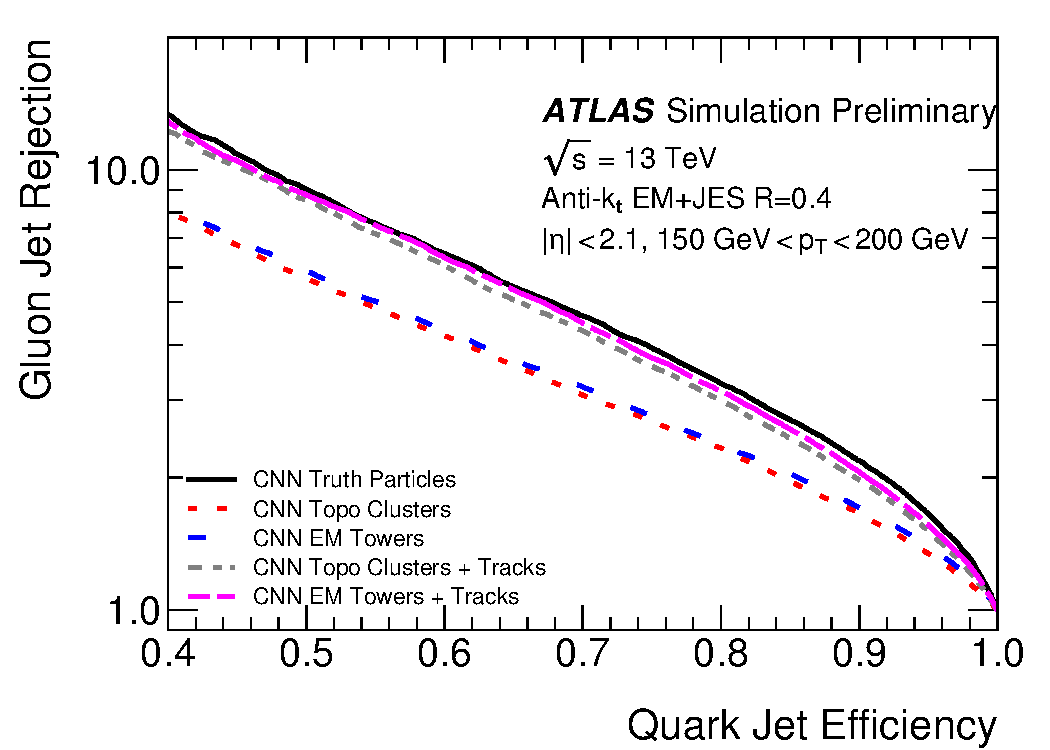
\includegraphics[width=0.5\textwidth]{figures/CNN/ROC_pt150_200_input.pdf}\label{lowpt}}
\subfloat[][]{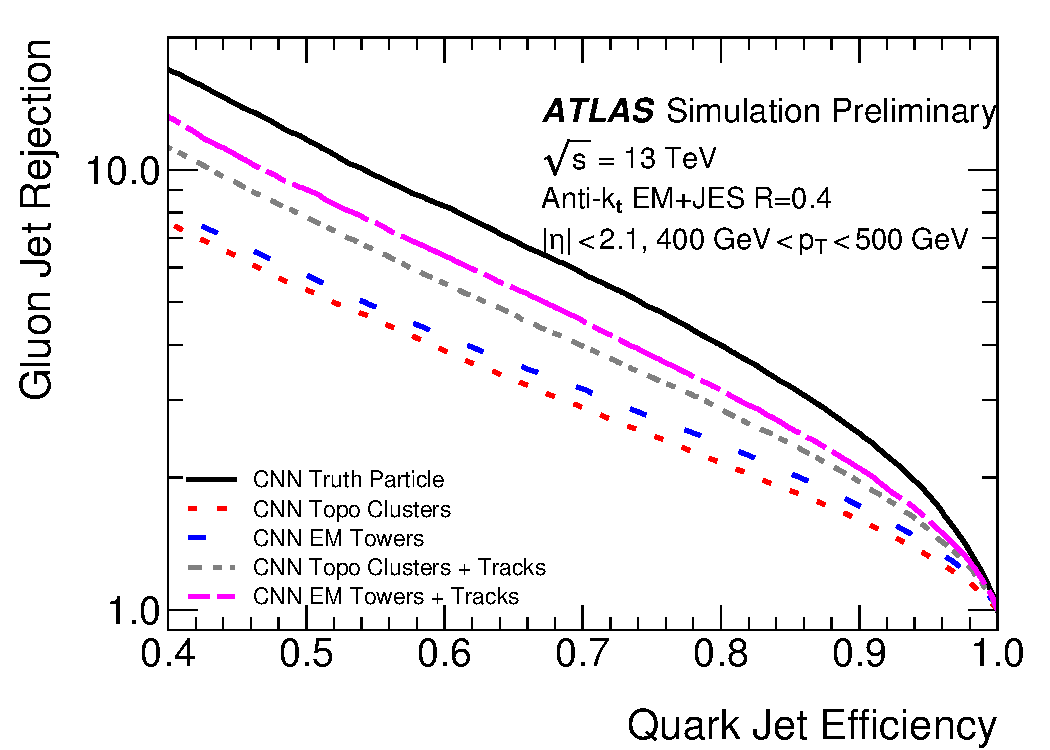
\includegraphics[width=0.5\textwidth]{figures/CNN/ROC_pt400_500_input.pdf}\label{highpt}}
\caption{Gluon jet rejection as a function of the quark jet efficiency using the CNN tagger with different inputs
for jets with \protect\subref{lowpt} $150<\pt<200~\GeV$ and \protect\subref{highpt} $400<\pt<500~\GeV$.}
\label{fig:cnn-input}
\end{center}
\end{figure}


%The difference between the full truth-particle line and the calorimeter + reconstructed tracks lines in Figure~\ref{fig:cnn-input} 
%depends on many details of the detector response, angular resolution, reconstruction efficiency, etc.  
%However, it is possible to isolate one component of the difference by focusing only on the charged-particles.  Figure~\ref{fig:cnn-tracktruth}(a) shows the performance of a track-only-image at both particle-level and detector-level.  As might be expected, due to the precise measurement of charged-particle trajectories, there is little difference between the particle- and detector-levels.  Degradation due to efficiency and resolution effects are only expected at much lower and higher transverse momenta.


\subsection{Detector Regions and Pile-ups}
\label{sec:cnn-detectorregion}

The robustness of the CNN q/g tagger is tested against experimental effects. In particular, the $\eta$ and pile-up effects are tested,
by training the tagger for the full range of different conditions and test tagger in a particular phase space.
For the jets considered in this study, part of them are fully within the barrel of the calorimeter $|\eta|<2.1$ and some of them
are in the barrel-endcap transition region $1.2<|\eta|<2.1$. As shown in Fig.\ref{fig:cnn-tracktruth} the $|\eta|$ dependence is negligible. 

%Both tower and topocluster inputs are projected onto a regular grid, but variations in the underlying geometry of the calorimeter could have an impact on performance.  
%Focusing on towers, Figure~\ref{fig:tracktruth}(b) shows that similar performance is achieved when testing the tagger on jets that are predominately in the barrel ($|\eta|<1.2$) 
%to those that are in the transition region between the barrel and endcap calorimeters ().
%The full $|\eta|$ range ($|\eta|<2.1$) is used for training.

\begin{figure}[htpb]
\begin{center}
 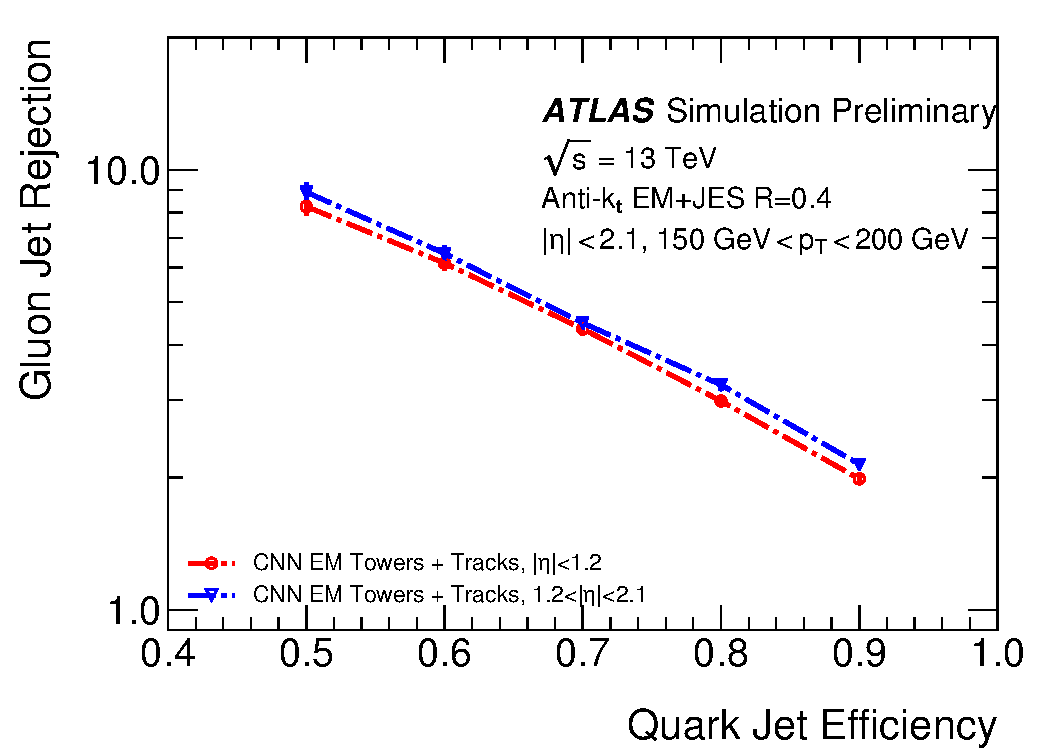
\includegraphics[width=0.6\textwidth]{figures/CNN/ROC_pt150_200_eta.pdf}
\caption{Gluon jet rejection as a function of the quark jet efficiency using the CNN tagger for jets with $150<\pt<200~\GeV$ in different $|\eta|$ regions}
%\protect\subref{tracktruth} Comparison between using track images and truth charge particle images as input.
%\protect\subref{kinematics} Comparison between different $|\eta|$ ranges. The full $|\eta|$ range ($|\eta|<2.1$) is used for training.}
\label{fig:cnn-tracktruth}
\end{center}
\end{figure}

The impact of pileup effects is also evaluated as the calorimeter tower image is subject to contamination from pile-ups
. The test sample is divided into both bins of $N_\text{PV}$
and bins of $\mu$. As shown in Fig.~\ref{fig:cnn-pileup} and \ref{fig:cnn-pileup2}, the tagger is robust against
to in-time ($N_\text{PV}$) as well as out-of-time pile-up ($\mu$) variations.

\begin{figure}[htpb]
\begin{center}
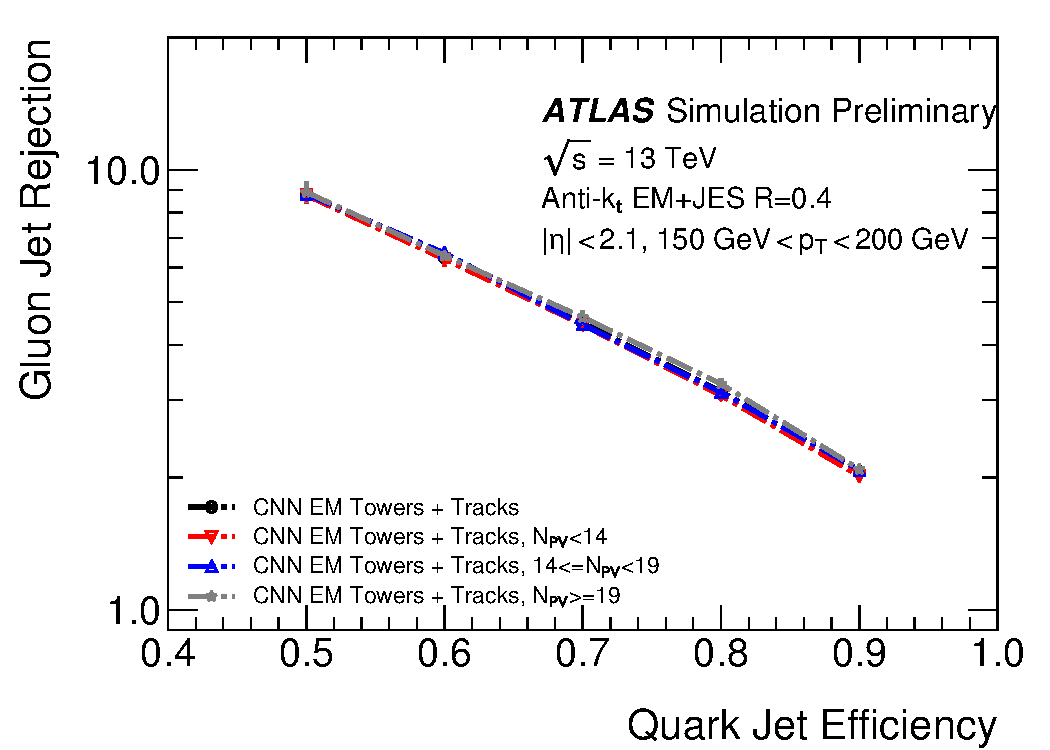
\includegraphics[width=0.6\textwidth]{figures/CNN/ROC_pt150_200_NPV.pdf}
\caption{Gluon jet rejection as a function of the quark jet efficiency %\protect\subref{roc} 
evaluated at different pileup conditions, 
quantified by the number of reconstructed primary vertices ($N_\text{PV}$).}
\label{fig:cnn-pileup}
\end{center}
\end{figure}

%Calorimeter-based discrimination is not only effected by in-time pileup (quantified by $N_\text{PV}$) but also by out-of-time pileup. 
%Figure~\ref{fig:cnn-pileup2} compares the tagger performance in two different regimes of the average number of collisions per bunch crossing ($\mu$) regimes corresponding to the out-of-time pileup representative of LHC Run 2 conditions.

\begin{figure}[htpb]
\begin{center}
\subfloat[][]{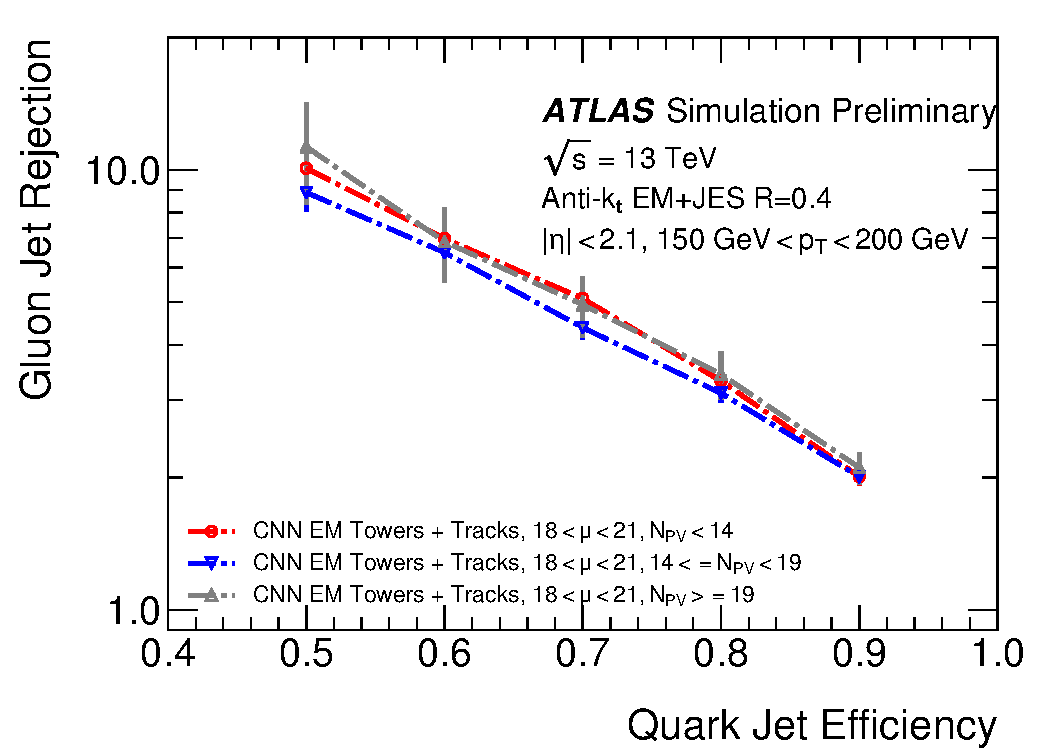
\includegraphics[width=0.5\textwidth]{figures/CNN/ROC_pt150_200_mu18_21.pdf}\label{roc1}}
\subfloat[][]{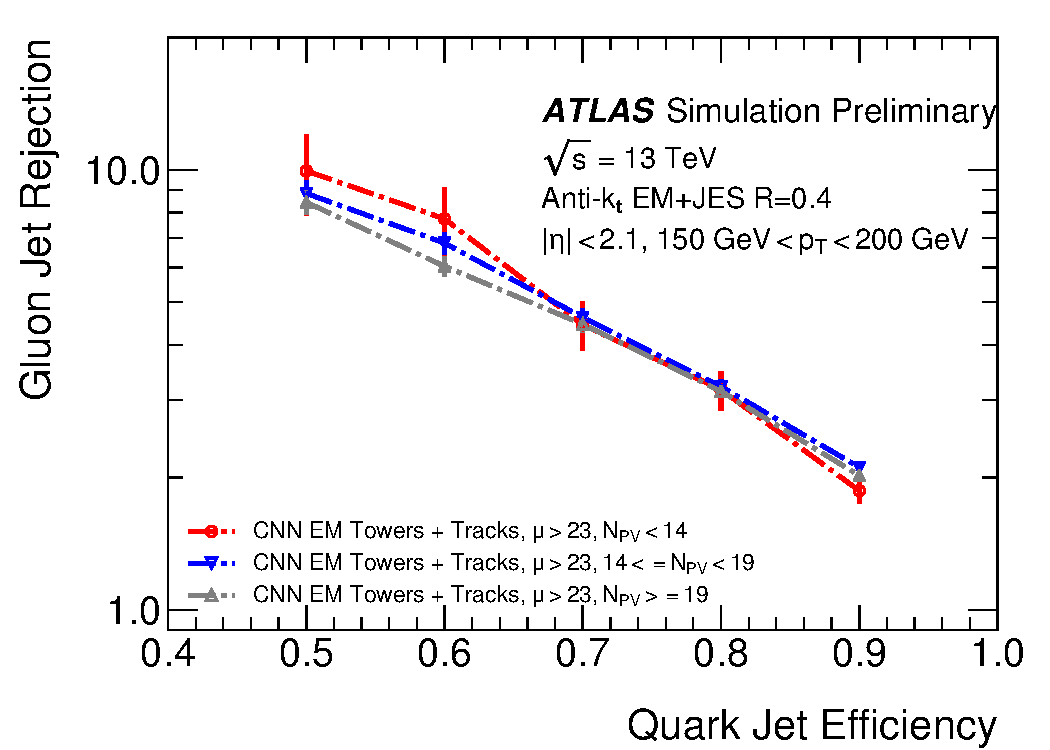
\includegraphics[width=0.5\textwidth]{figures/CNN/ROC_pt150_200_mu23.pdf}\label{roc2}}
\caption{Gluon jet rejection as a function of the quark jet efficiency 
evaluated at different levels of $N_\text{PV}$ for \protect\subref{roc1} $18<\mu<23$ and \protect\subref{roc2}  $\mu > 23$.
The two $\mu$ bins where chosen to have roughly the same number of events.}
\label{fig:cnn-pileup2}
\end{center}
\end{figure}


\subsection{Modeling}

Fragmentation modeling could affect significantly the descriptions of quark and gluon jets and hence
the performance of the CNN q/g tagger.
Figure~\label{fig:cnn-avg:CNN} shows that the average image of quark and gluon jets simulated in 
\textsc{Pythia} 8 and with \textsc{Herwig++}. It is noteworthy that there is a more significant difference between
quark and gluon jets in \textsc{Pythia} 8 images as compared to that of \textsc{Herwig++}. Such difference mainly comes
from the description of the quark jets. 

%The radiation pattern inside gluon jets is similar between the two models, whereas there are larger differences for quark jets.  
%In particular, quark and gluon jets are more different according to  relative to 
%This is observed with the CNN in Fig.~\ref{fig:cnn-pythiasherpa}.
%As gluon jets in \textsc{Herwig++} are more similar to quark jets than in \textsc{Pythia} 8, 
%any observable (including the CNN tagger output) tends to have less discrimination power when tested in \textsc{Herwig++}.

Although the images from \textsc{Pythia} 8 and \textsc{Herwig++} are different
we still want to know if the CNN tagger trained with these different images
would still learn the physics difference between quark and gluon jets. Following the study
of ~\cite{Barnard:2016qma}, two networks are separately trained with \textsc{Pythia} 8 and \textsc{Herwig++}
images and each of them is then tested on \textsc{Pythia} 8, \textsc{Sherpa} and \textsc{Herwig++}
images. We noticed that the if the same network is used for testing and only the training sample is varied, 
the performance gap is small (consistent with the result from ~\cite{Komiske:2016rsd}) while the difference is large
if the testing samples are different (mainly between \textsc{Pythia} and \textsc{Herwig++}).
Hence the network is robust against the different fragmentation models and gives
us the confidence applying the MC trained networks to data. Also, not surprisingly, since \textsc{Sherpa} employs similar fragmentation
model as \textsc{Pythia}, the CNN tagger is essentially indifferent to these two models.

\begin{figure}[htpb]
\begin{center}
  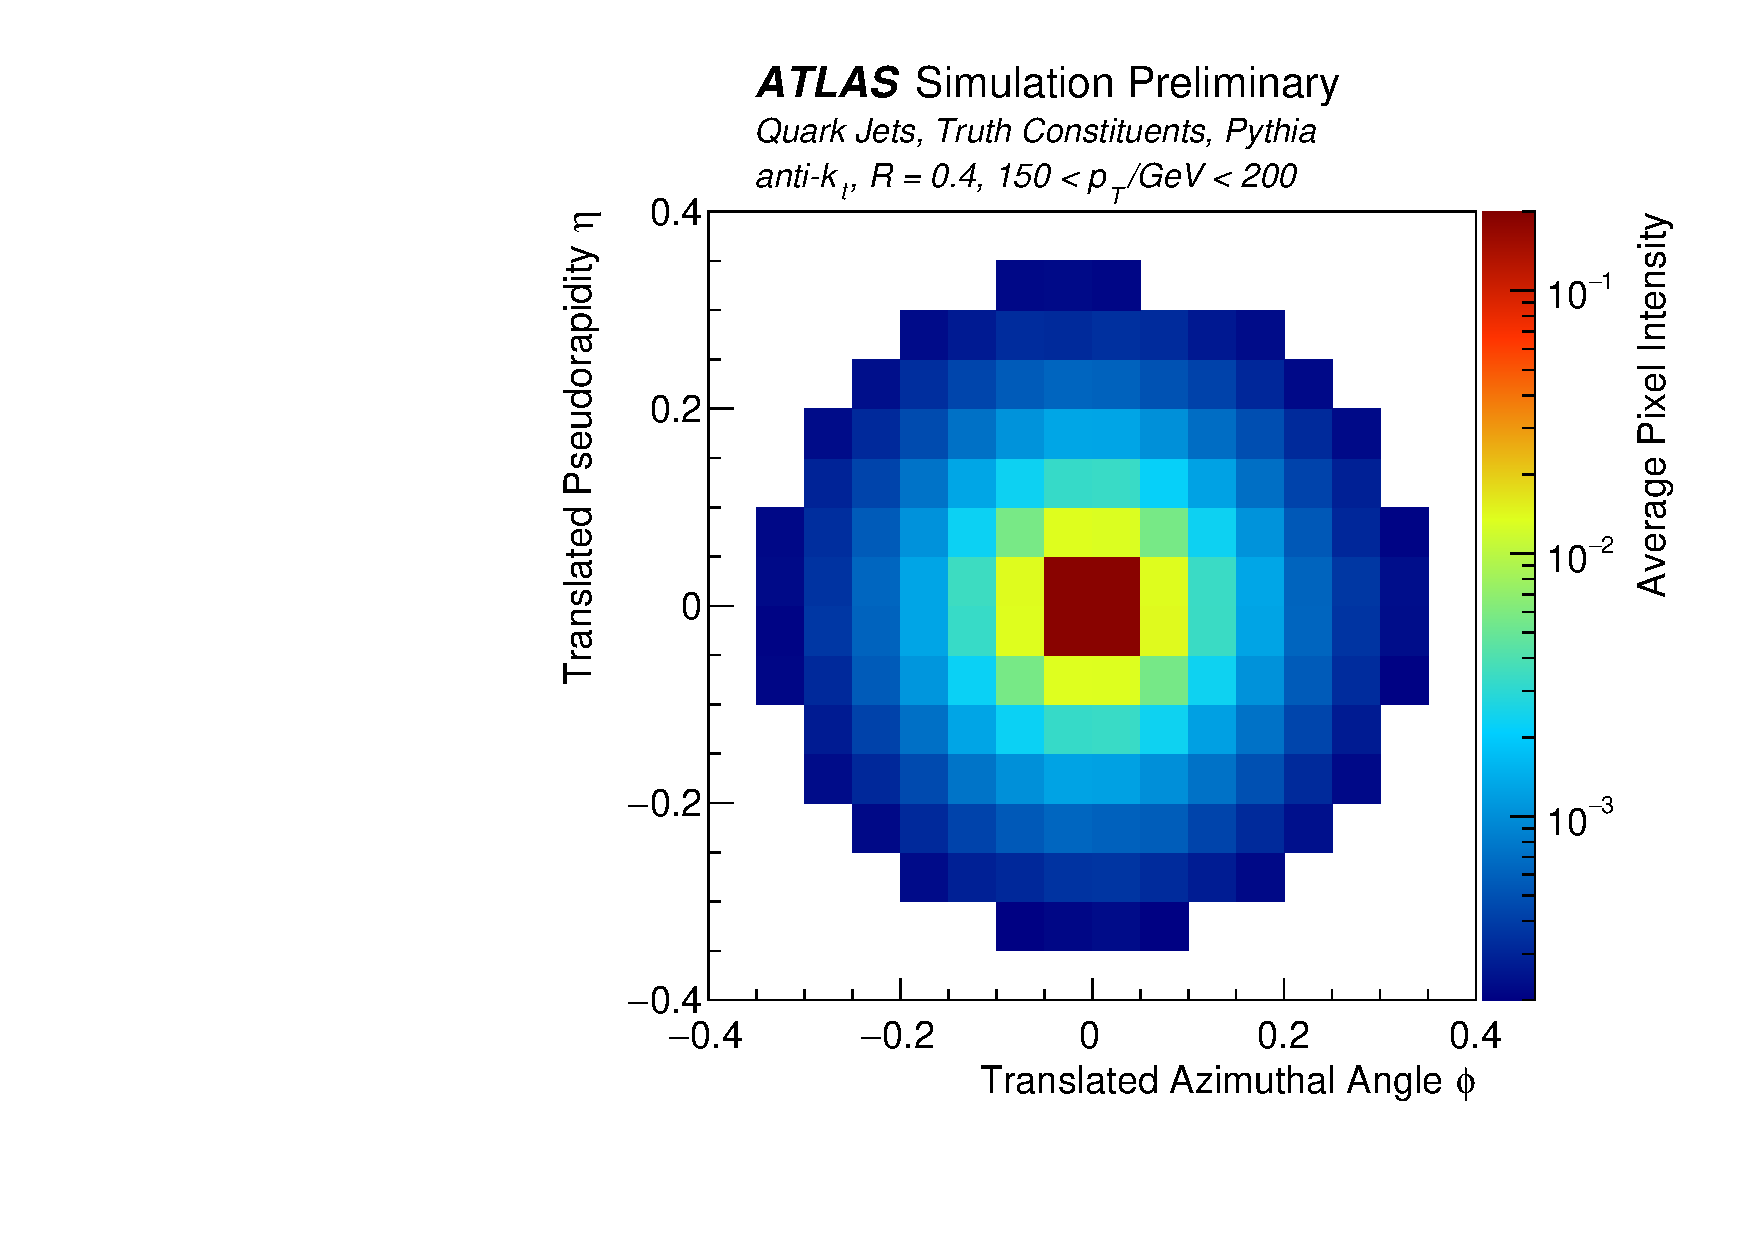
\includegraphics[width=0.31\textwidth]{figures/CNN/quark_truth_pythia.pdf}
  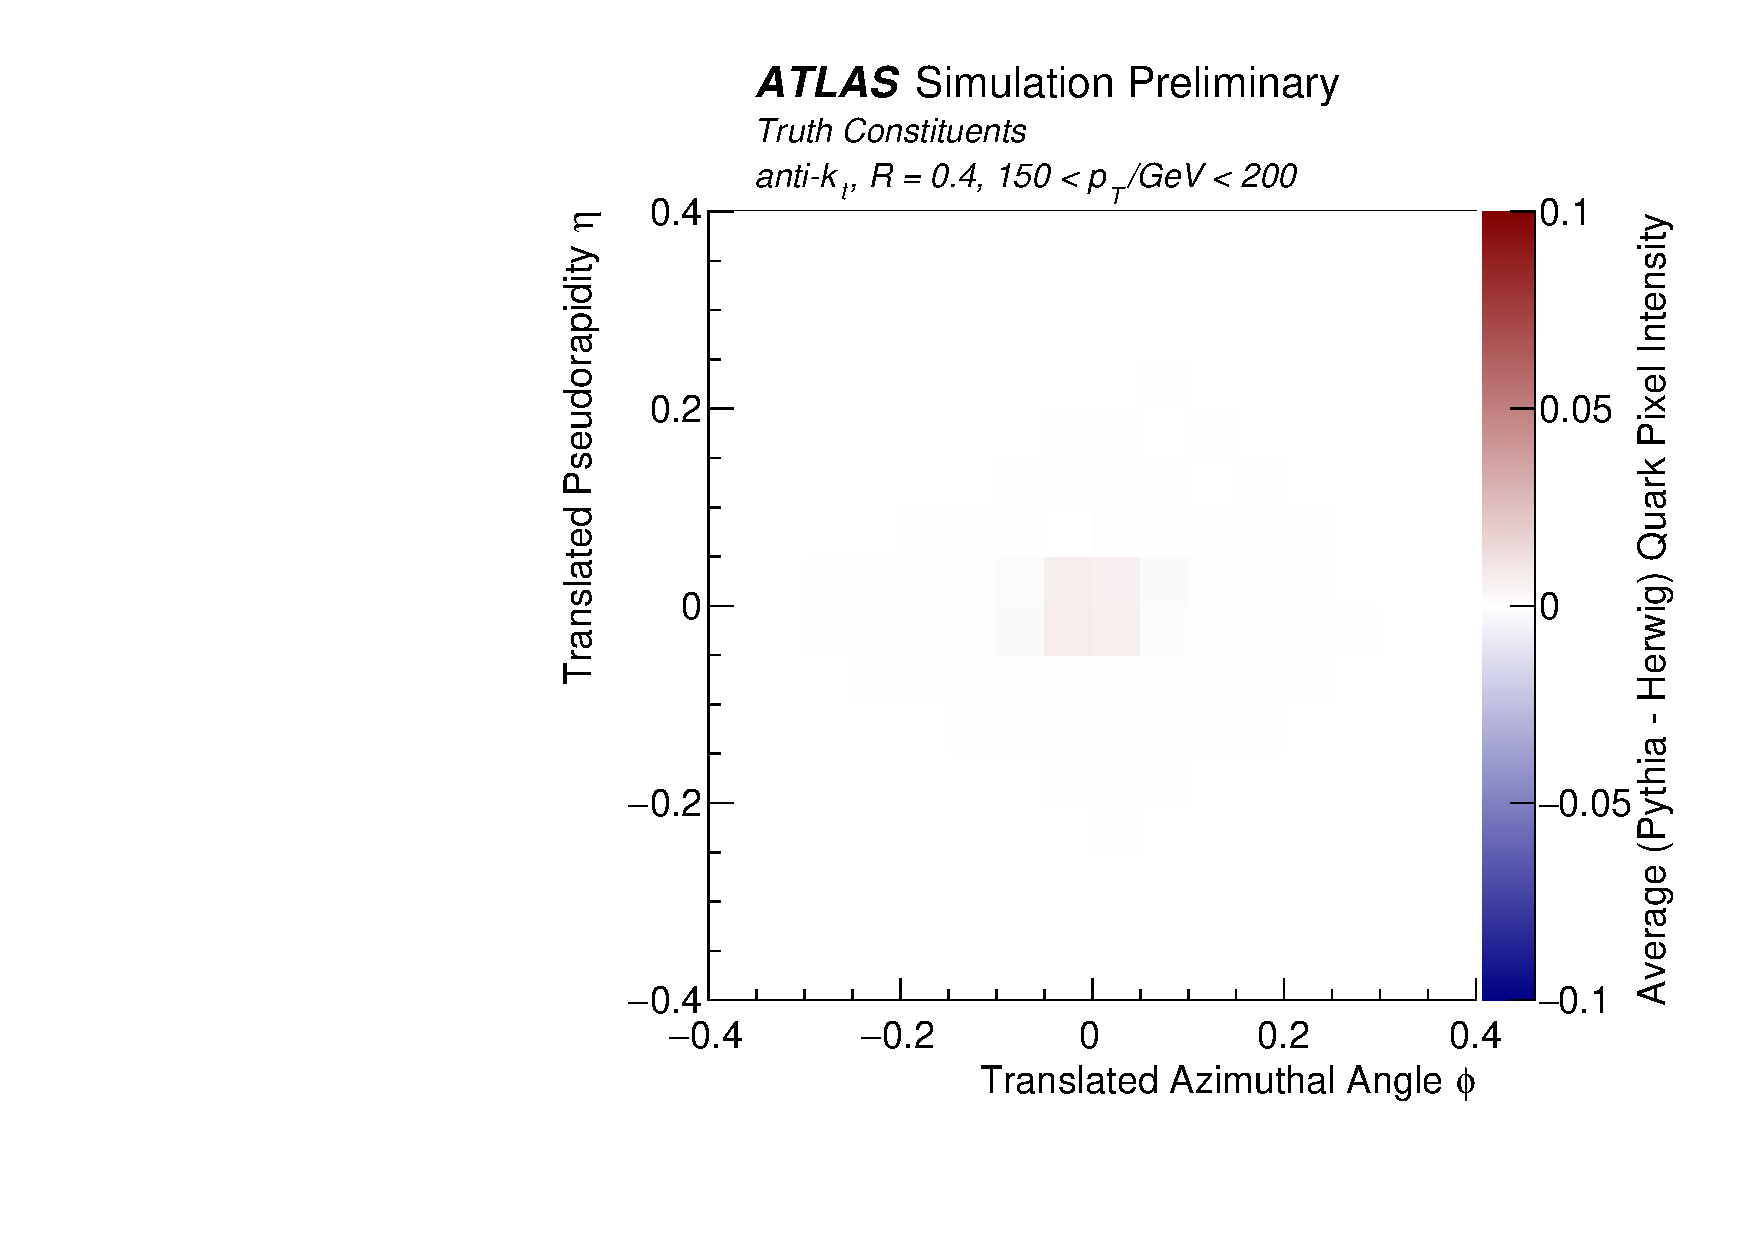
\includegraphics[width=0.31\textwidth]{figures/CNN/diff_truthq_pythiaherwig.pdf}
  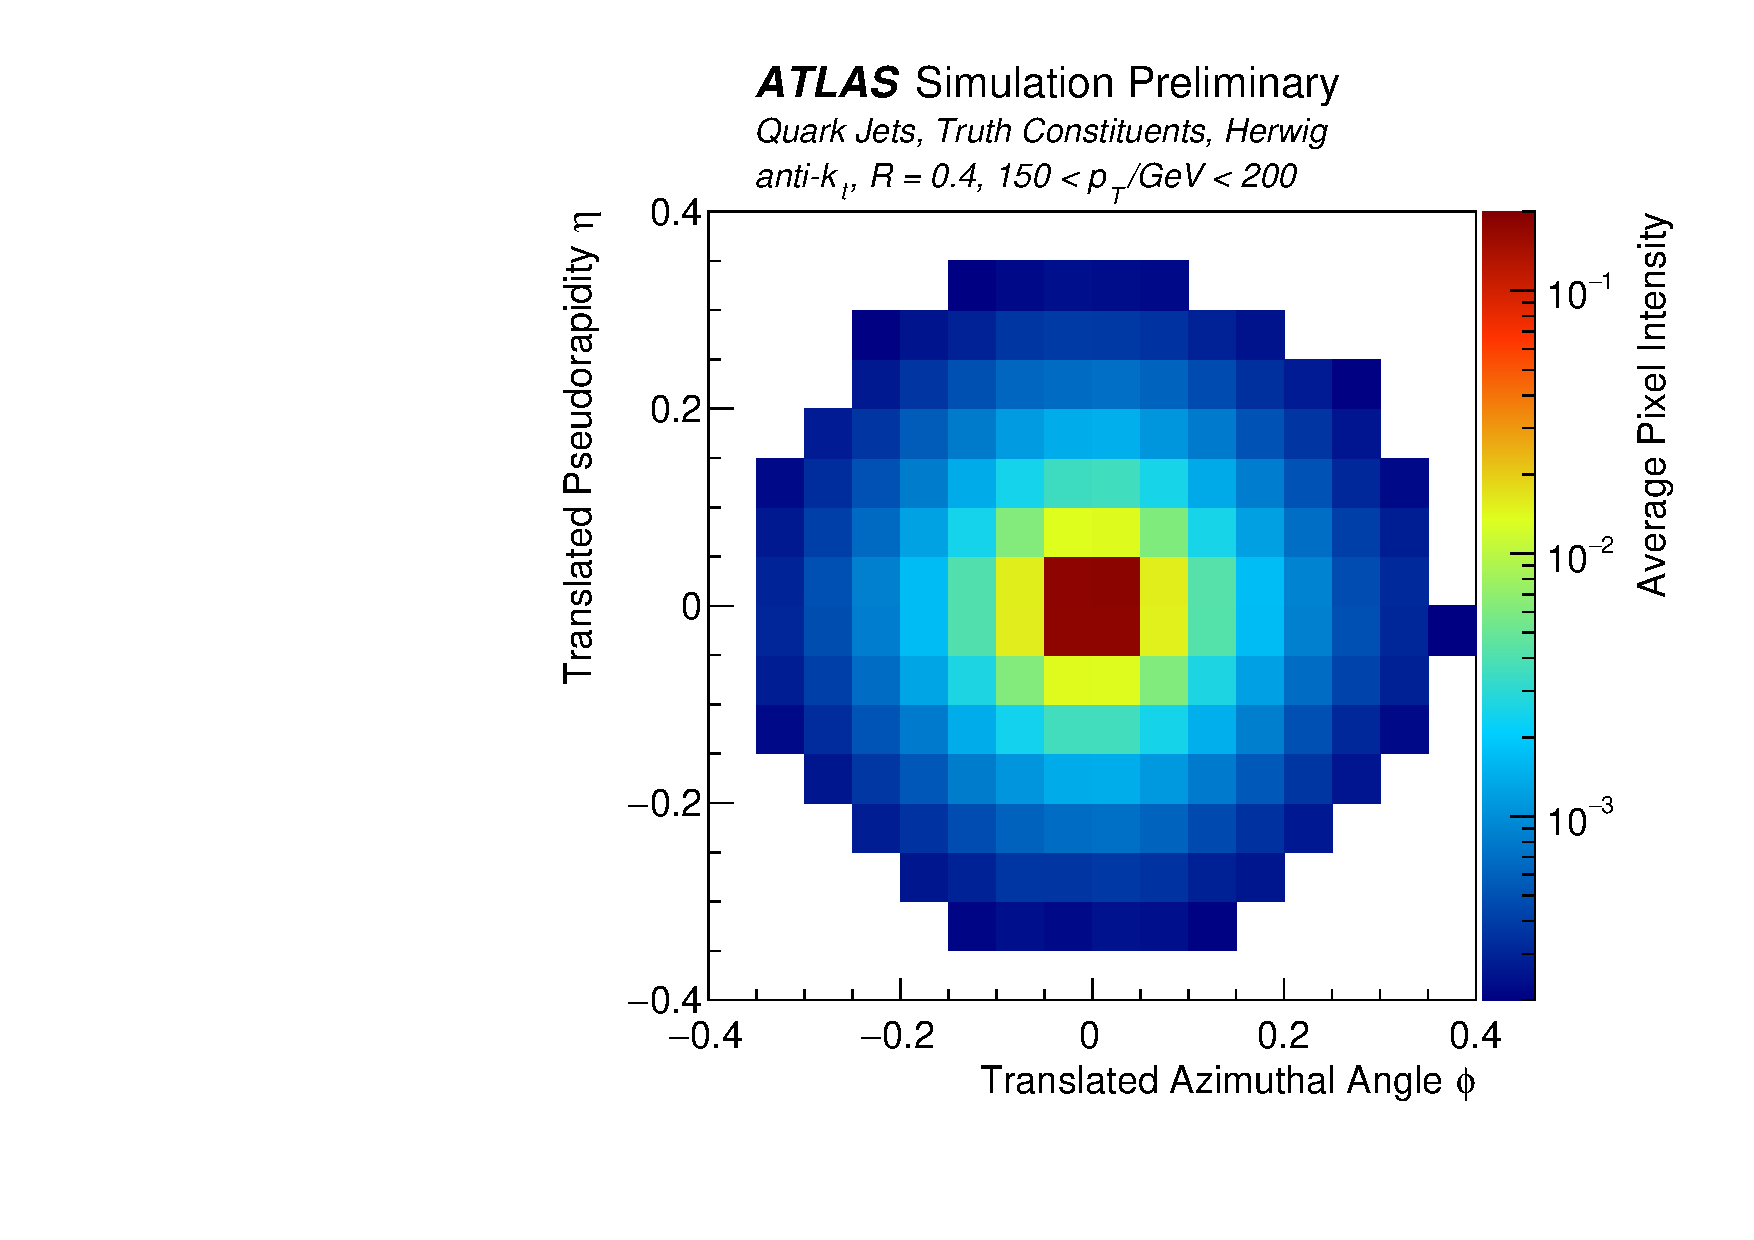
\includegraphics[width=0.31\textwidth]{figures/CNN/quark_truth_herwig.pdf}\\
  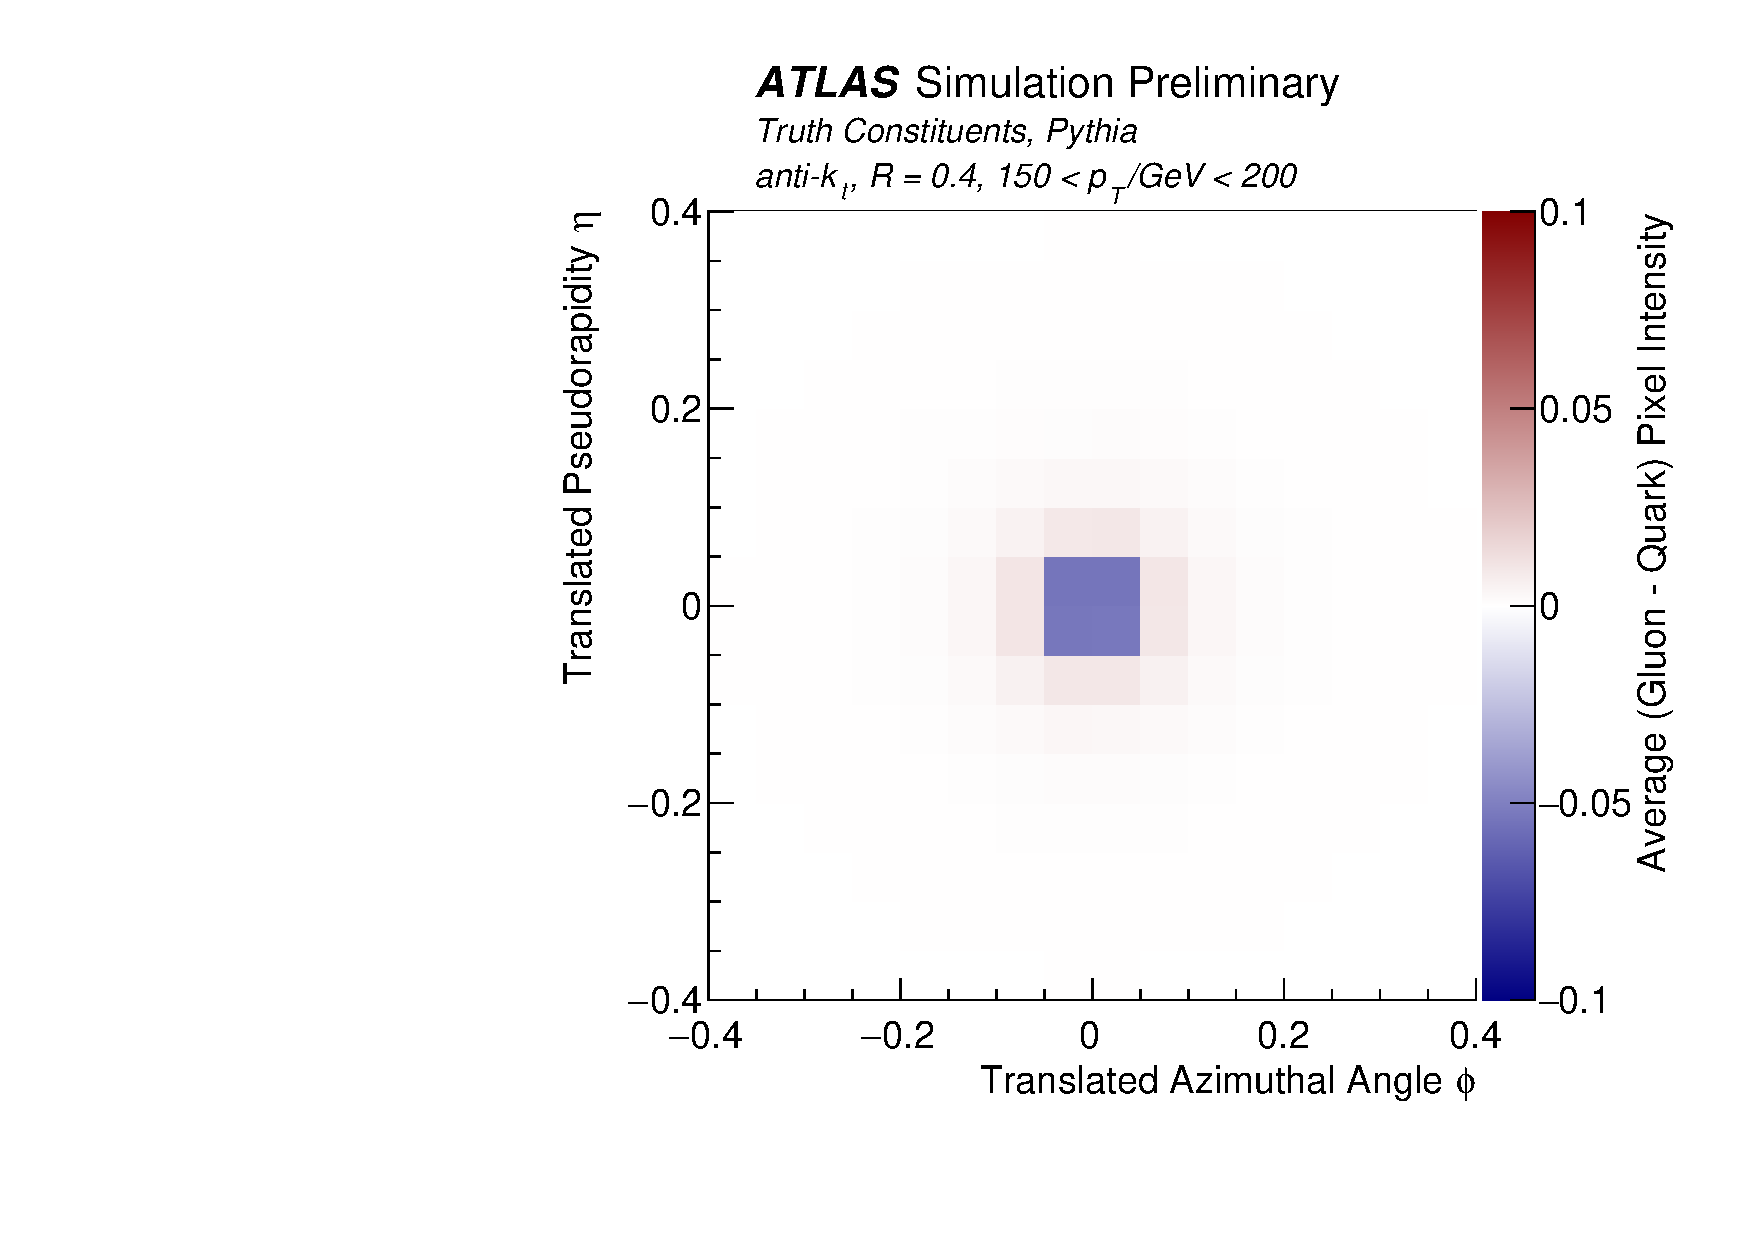
\includegraphics[width=0.31\textwidth]{figures/CNN/diff_truth_pythia.pdf}\hspace{54mm}
  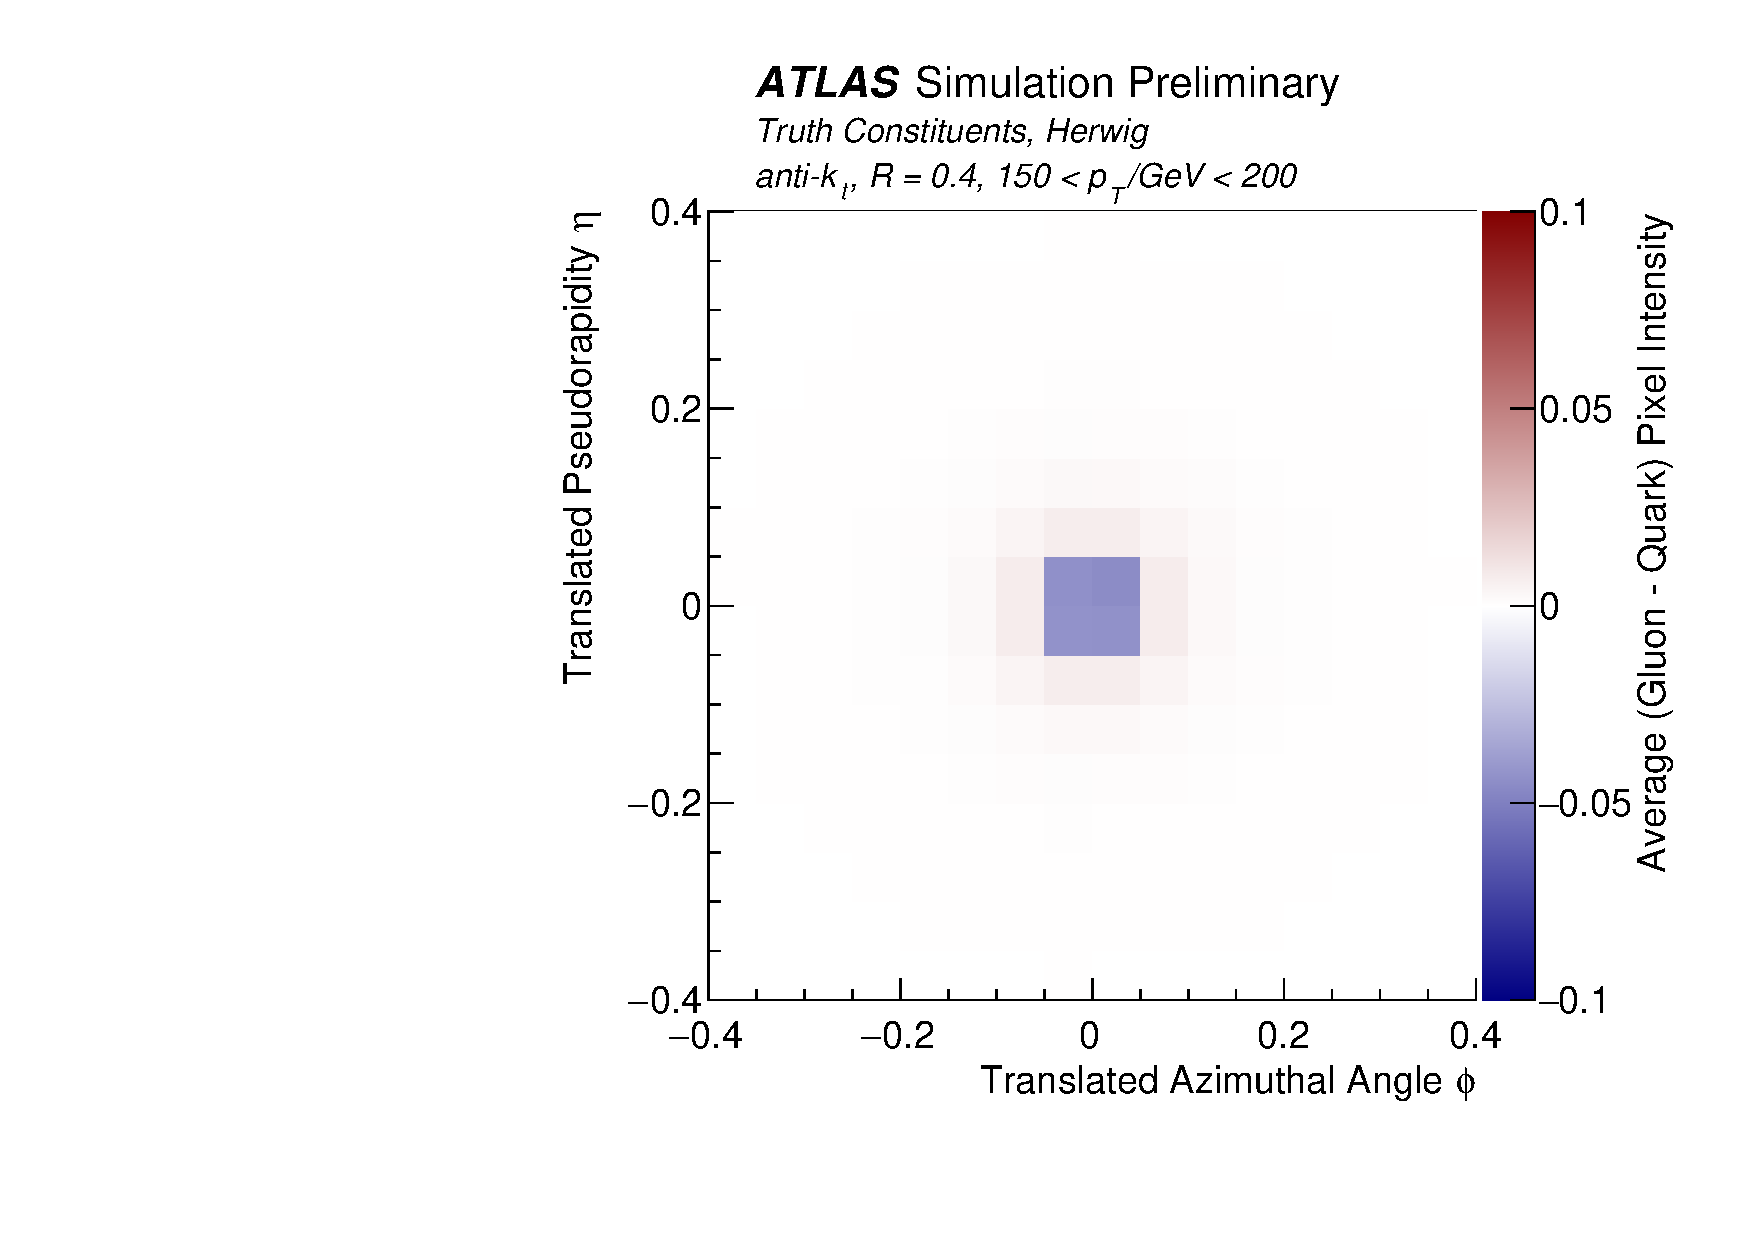
\includegraphics[width=0.31\textwidth]{figures/CNN/diff_truth_herwig.pdf}\\
  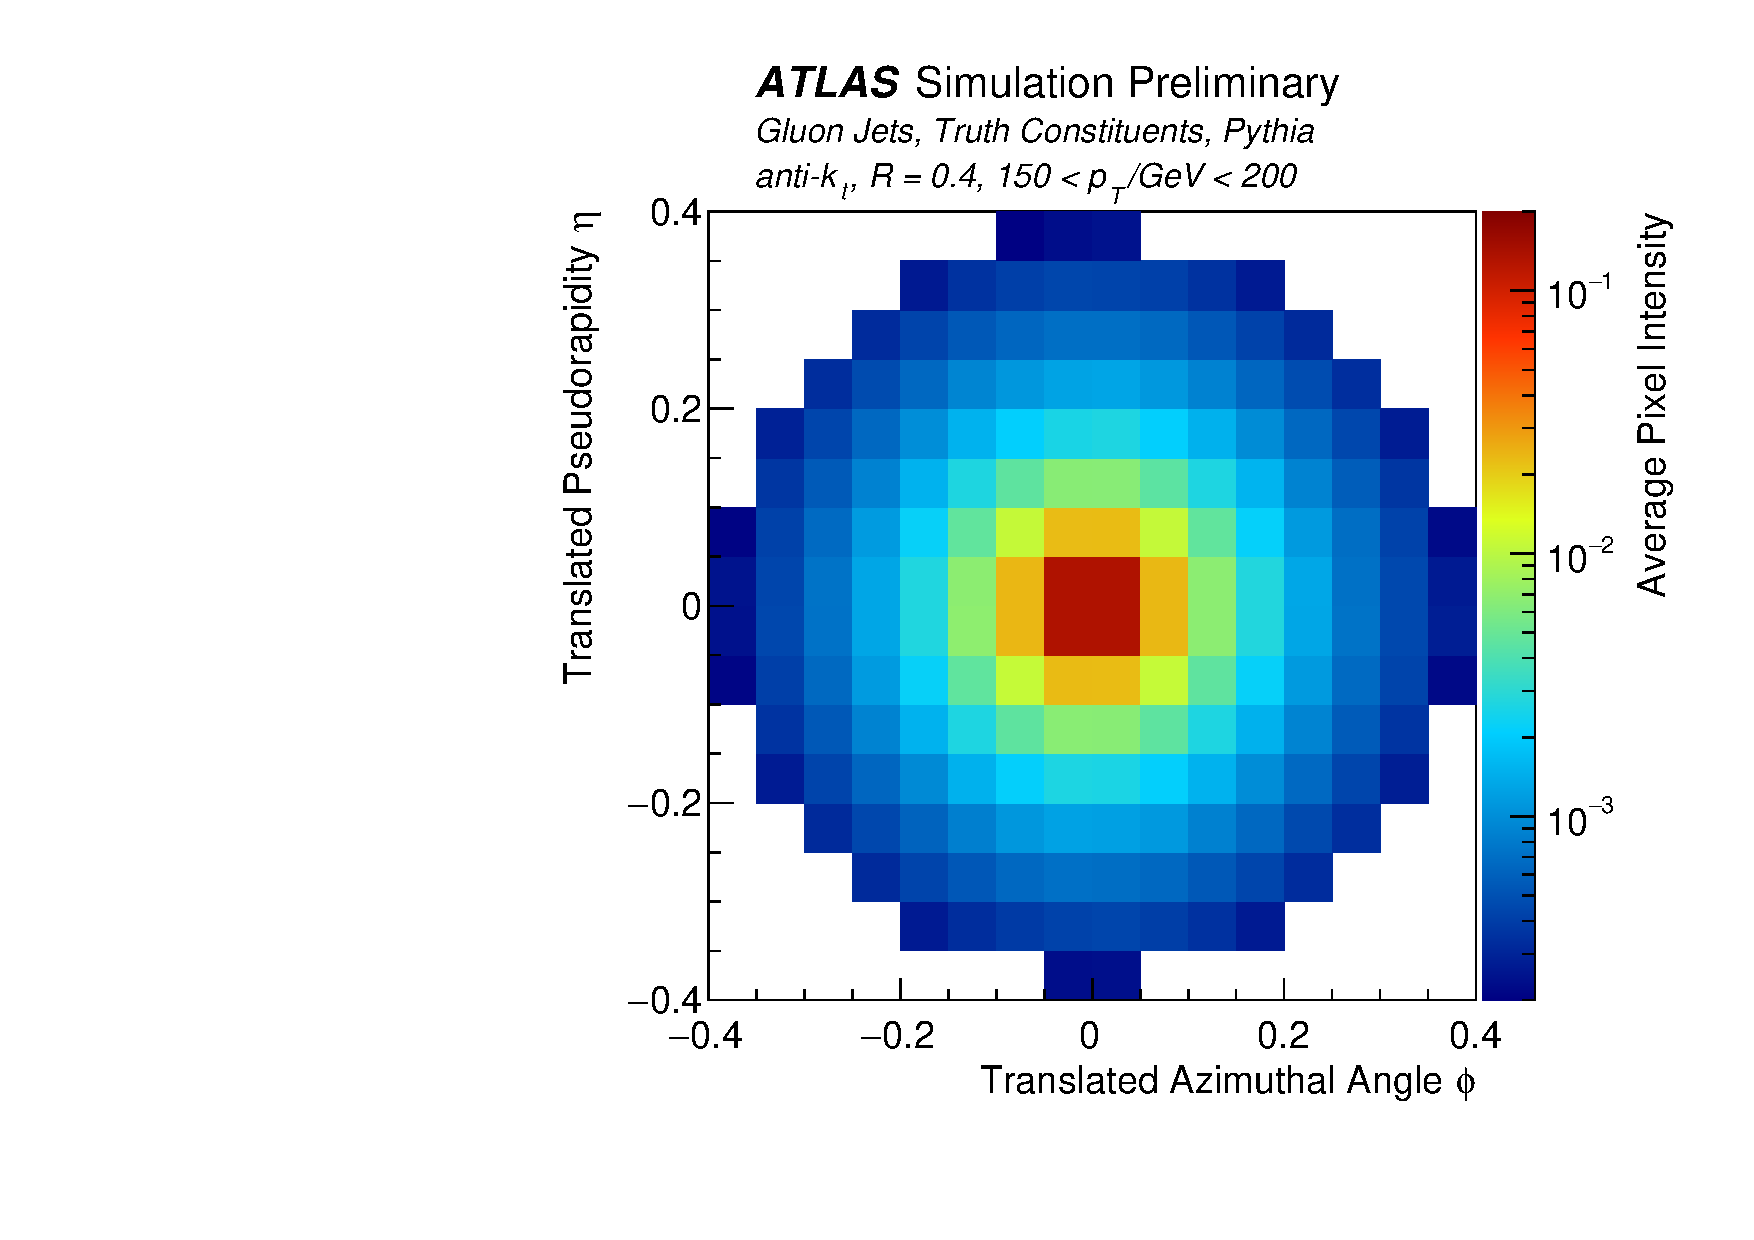
\includegraphics[width=0.31\textwidth]{figures/CNN/gluon_truth_pythia.pdf}
  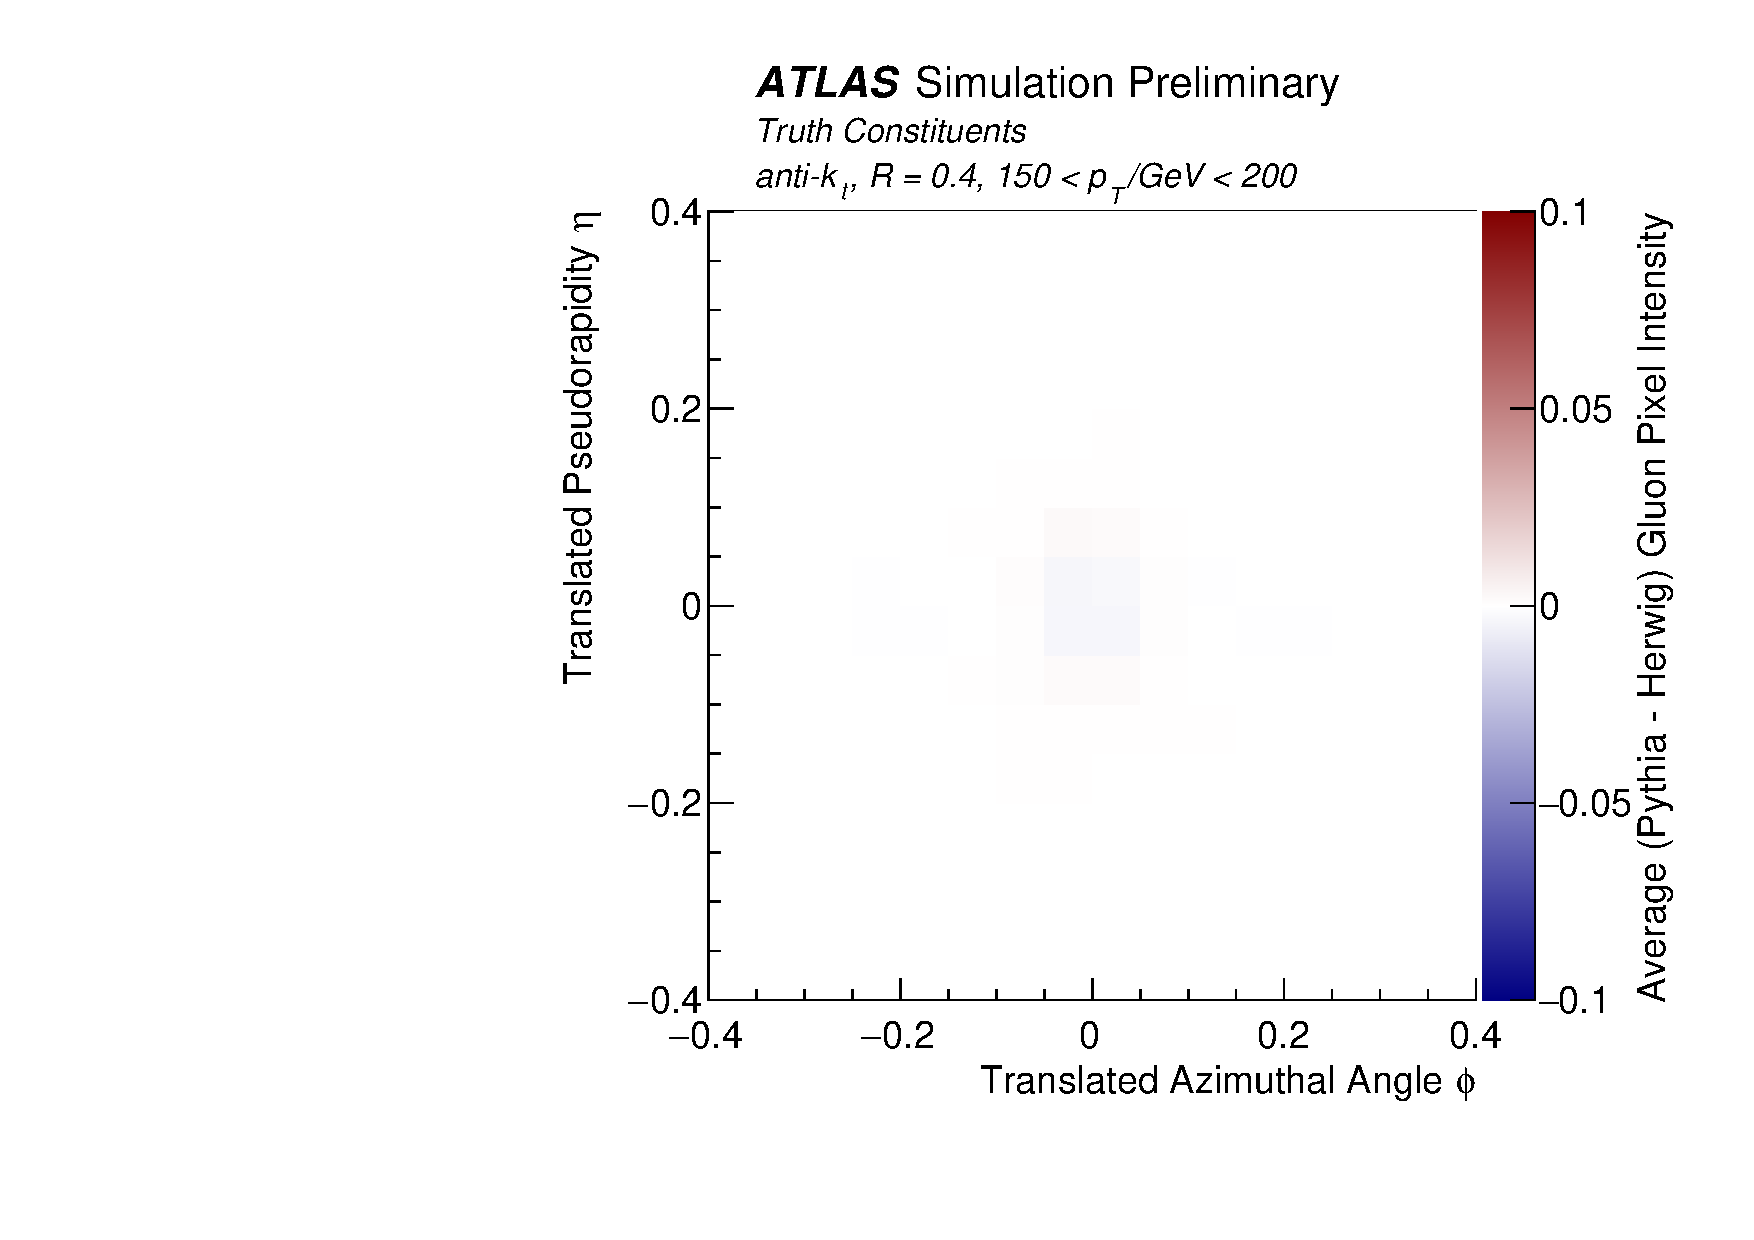
\includegraphics[width=0.31\textwidth]{figures/CNN/diff_truthg_pythiaherwig.pdf}
  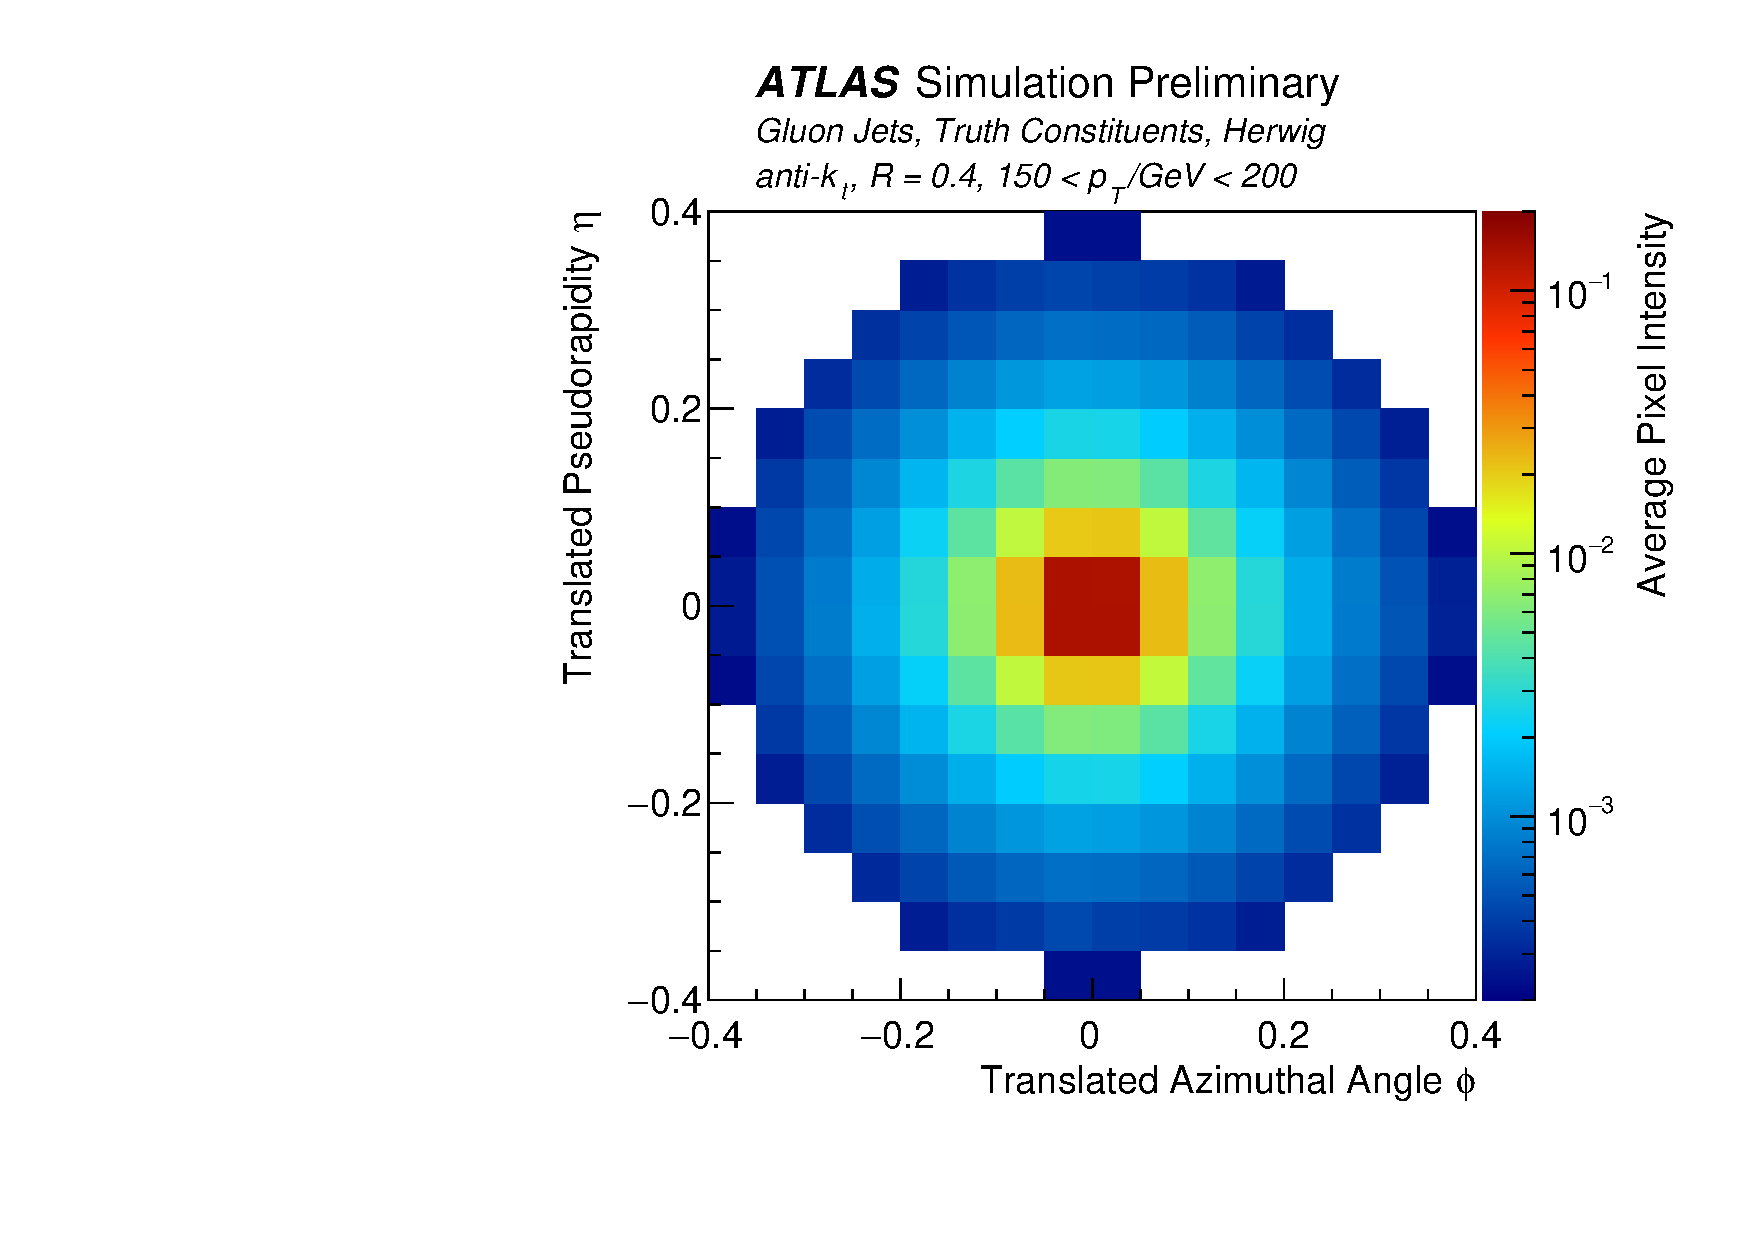
\includegraphics[width=0.31\textwidth]{figures/CNN/gluon_truth_herwig.pdf}
\caption{
The four corners show the average quark (top) and gluon (bottom) jet images, for jets generated with \textsc{Pythia} (left) and
and \textsc{Herwig} (right); the four plots on the edges show the difference between the adjacent plots,
for example the top plot shows the difference between the average quark jet in \textsc{Pythia} and
and \textsc{Herwig}.}
\label{fig:cnn-avg:CNN}
\end{center}
\end{figure}


\begin{figure}[htpb]
\begin{center}
\subfloat[][]{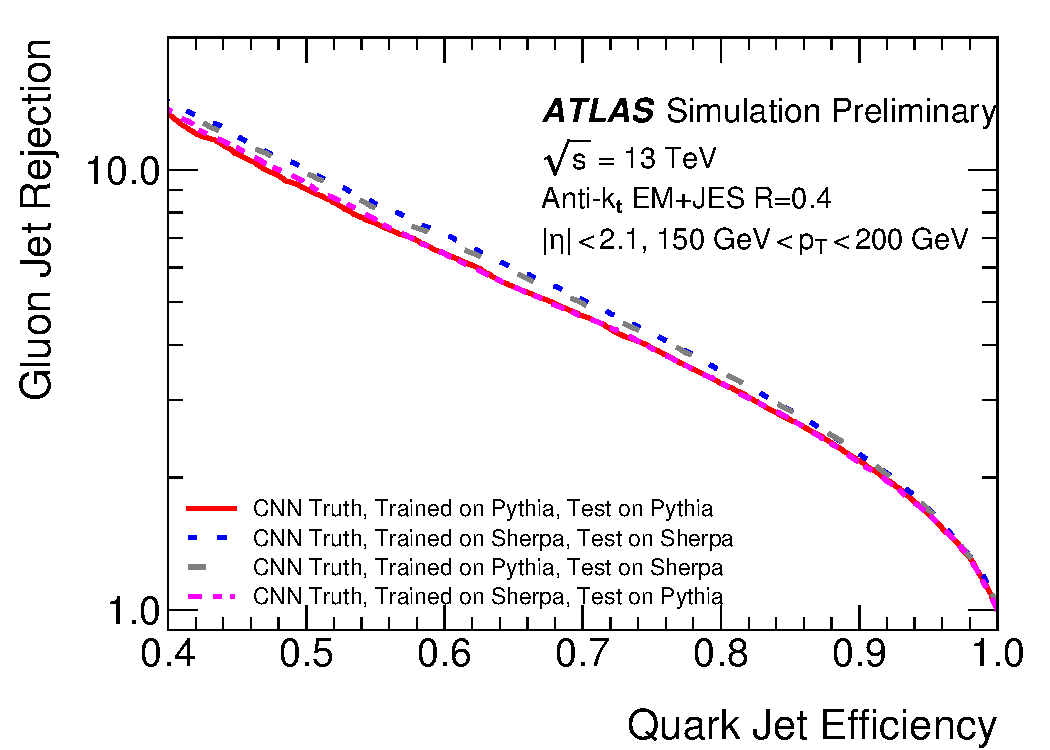
\includegraphics[width=0.5\textwidth]{figures/CNN/ROC_pt150_200_gen_pythia_sherpa.pdf}\label{CNN}} 
\subfloat[][]{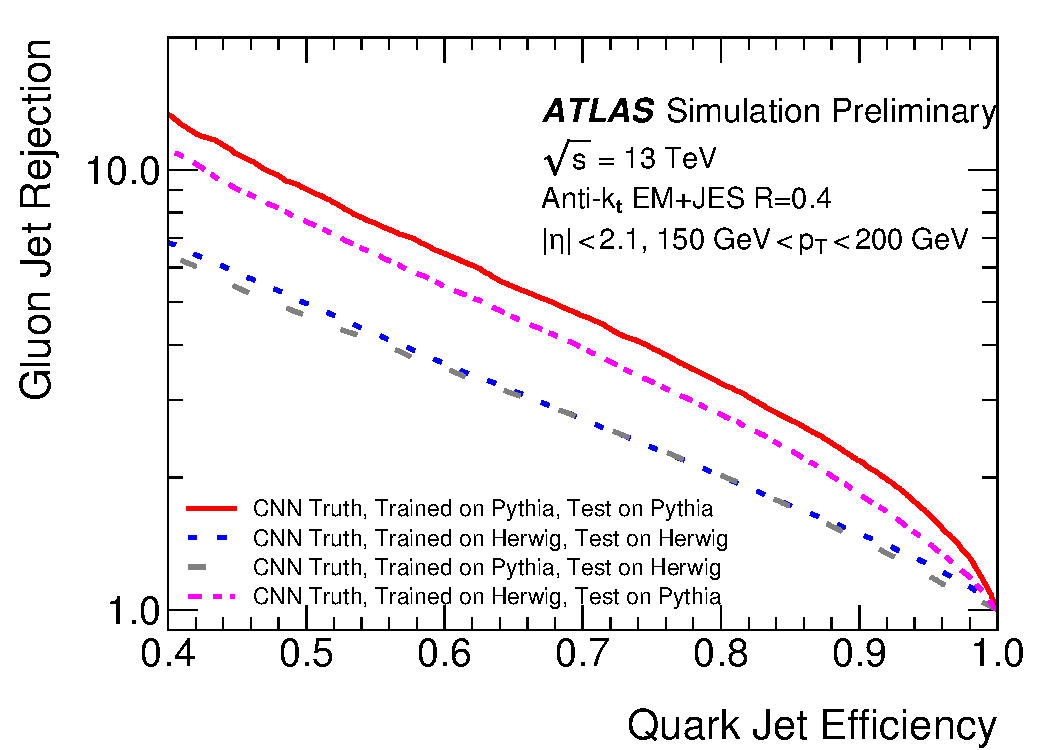
\includegraphics[width=0.5\textwidth]{figures/CNN/ROC_pt150_200_gen_pythia_herwig.pdf}\label{pythiaherwig}} 
\caption{Gluon jet rejection as a function of the quark jet efficiency comparing \textsc{Pythia} to \protect\subref{CNN} \textsc{Sherpa}
and \protect\subref{pythiaherwig} \textsc{Herwig} for jets with $150<\pt<200~\GeV$.}
\label{fig:cnn-pythiasherpa}
\end{center}
\end{figure}
